\documentclass[FM,BP]{tulthesis}

\usepackage[czech]{babel}
\usepackage[utf8]{inputenc}
\usepackage[a-1a]{pdfx}
\usepackage{hyperref}
\usepackage{amsmath}
\usepackage{amssymb}
\usepackage{nicefrac}
\usepackage{caption}
\usepackage{listings}

\usepackage[titles]{tocloft}
\usepackage[titletoc,title]{appendix}
\newcounter{Vzorce}
\addtocounter{Vzorce}{1}

\TULtitle{Řešení optimalizační úlohy LASSO pomocí proximálních algoritmů}{Solution to LASSO Using Proximal Algorithms}
\TULprogramme{B2646}{Informační technologie}{Information Technology}
\TULbranch{1802R007}{Informační technologie}{Information Technology}
\TULauthor{Václav Langr}
\TULsupervisor{doc. Ing. Zbyněk Koldovský, Ph.D.}

\begin{document}
\ThesisStart{male}{zadan}
\begin{acknowledgement}
Chtěl bych tímto poděkovat všem, kteří mne podporovali. Především mé rodině za velikou podporu, díky které mi bylo umožněno studovat. \\ Zároveň bych chtěl poděkovat také vedoucímu této práce doc. Ing. Zbyňku Koldovskému, Ph.D. za velice přínosné konzultace, rady a trpělivost.
\end{acknowledgement}
\clearpage
\begin{abstractCZ}
Tato bakalářská práce je zaměřena na rekonstrukci řídkého vektoru z jeho komprimovaného pozorování. Pro rekonstrukci se využívá optimalizačního problému LASSO a jeho řešení pomocí proximálních algoritmů. Po vytvoření takového algoritmu, který je schopen původní signál rekonstruovat, se využívá metody Monte Carlo pro pozorování závislosti chyby řešení na parametru lambda. Pro takto získaný výpočet je zjištěna kvadratická chyba řešení LASSO od původního vektoru dat, která je následně porovnávána s teoretickou chybou.


Vypracování této bakalářské práce bylo rozděleno do několika navazujících částí. Prvním a také nejdůležitějším krokem bylo nastudování vlastností proximálních algoritmů a výpočet proximálního operátora při různých vstupních funkcích. Po takto provedené rešerši proximálních algoritmů proběhla také rešerše vlastností optimalizační úlohy LASSO a jejích variant. Následně bylo možné přistoupit k implementaci algoritmu v programovacím jazyce a vývojovém prostředí MATLAB. Při postupné implementaci byl algoritmus upraven tak, aby vždy zkonvergoval ke správnému nebo alespoň velice přesnému přibližnému řešení optimalizačního problému. Z tohoto důvodu byl algoritmus rozšířen o podmínky optimality, jež ukončují výpočet při dosažení poměrně přesné aproximace. Dále byl rozšířen o výpočet dynamické velikosti kroku. S takto připraveným algoritmem mohla být vytvořena metoda Monte Carlo, která generuje nekomprimovaný řídký vektor dat, měřící matice, jejichž prvky mají Gaussovo rozložení, a parametr lambda v zadaném rozsahu s logaritmickým rozdělením.    


Výsledek této práce může být využit pro další zpracování. Jedním z možných použití je např. pro vytvoření nového datového formátu, ve kterém by byl uložen jen komprimovaný vektor dat případně i měřící matice, pokud by nebyla shodná pro všechny komprimace. Na straně klienta by byl tedy pouze zrekonstruován původní nekomprimovaný signál.


\textbf{Klíčová slova:} MATLAB, proximální algoritmus, proximální operátor, LASSO, Monte Carlo
\end{abstractCZ}
\vspace{2cm}
\begin{abstractEN}
This bachelor thesis is focused on reconstruction of sparse vector from his compressed observation. For the reconstruction is used the LASSO problem and its solution using proximal algorithms. After creation of an algorithm that is able to restore the original signal is used Monte Carlo method for analyzing dependence of computation error on lambda parameter. Then is calculated the squared error for the found solution and the original data that is compared with the theoretical error.


Realization of this bachelor thesis was divided into several parts. The very first and the most important step was studying the properties of proximal algorithms and evaluation of proximal operator for different functions. After the research on proximal algorithms there was also research on the properties of the LASSO and its variants. After that is was possible to implement algorithm using MATLAB language and development environment. The algorithm was modified during the implementation so it always converges into correct or at least approximate solution of LASSO. Due to this reason optimality conditions were added that terminates solving if the approximation is very accurate and a computation of dynamical step size. This prepared algorithm could be used for creation of Monte Carlo method that generates uncompressed sparse vector of data, random measurement matrix with Gaussian distribution and a lambda parameter within an interval with logarithmic distribution.


The result of this thesis can be used for another usage. One of the possible usage is for example creation of a new data format. The compressed data would be saved in this format and only if the measurement matrix is not the same for all compressions it would be also saved. On the client side the original uncompressed signal would be recovered.


\textbf{Keywords:} MATLAB, Proximal Algorithm, Proximal Operator, LASSO, Monte Carlo
\end{abstractEN}
\clearpage
\tableofcontents

\listoffigures

\newcommand{\listequationsname}{Seznam vzorců}
\newlistof{myequations}{equ}{\listequationsname}
\newcommand{\myequations}[1]{%
	\addcontentsline{equ}{myequations}{\protect\numberline{}#1}\par}
\setlength{\cftmyequationsnumwidth}{0.0em}
\listofmyequations

\pagebreak

\renewcommand{\baselinestretch}{1.50}
\setlength\parindent{1.2cm}
\selectfont

\chapter{Úvod}
\label{ch:uvod}
 V dnešním světě, kdy získáváme stále více důležitých a velkých dat je stále důležitější nějakým způsobem získaná data komprimovat. Z tohoto důvodu se tato práce zabývá komprimací dat a následnou rekonstrukcí u koncového uživatele. Bude pro to použito nového přístupu pomocí proximálních algoritmů, které jsou rychlé a jednoduché na implementaci.

Základní měření odpovídá funkci, viz \ref{eq:Zakladni mereni}, kde jsou původní data $x_0 \in \mathbb{C}^n$ transformovány měřící maticí $A \in \mathbb{C} ^{m \times n}$, kde $m$ je počet řádků a $n$ počet sloupců matice a v poslední řadě je nutné uvažovat i náhodná data $z \in \mathbb{C}^m$, v našem případě toto reprezentuje náhodný šum. Takto jsou získaná nová data $y \in \mathbb{C}^m$. V obecných případech platí, že $m \geq n$, ale takto nedochází k žádné komprimaci dat případně by i vzrostl počet dat. Následná rekonstrukce by se tak redukovala pouze na spočtení inverzní, v případě obdélníkové matice pseudoinverzní, matice $A^{-1}$ a spočtení původních dat $x_0$. Tato bakalářská práce se zabývá případy, kdy $m < n$ a nelze tedy použít pseudoinverzní matici.

\begin{equation} \label{eq:Zakladni mereni} \tag{Vzorec \theVzorce}
y = A \times x_0 + z
\end{equation}
\myequations{\ref{eq:Zakladni mereni} - Základní měření}
\stepcounter{Vzorce}

Dle pravidel lineární algebry tak existuje nekonečně mnoho řešení a je tak nemožné v tomto případě zrekonstruovat původní data. Nicméně ve skutečnosti lze data zrekonstruovat a to za podmínky, že původní vektor dat $x_0$ je řídký, tedy většina prvků z $x_0$ je rovno $0$. Právě z tohoto důvodu jsou kompresní algoritmy, například pro kompresi formátu JPEG, kdy se ukládají pouze největší koeficienty diskrétní kosinové transformace, tak efektivní. Toto ale není jediná podmínka, nutná k úspěšné rekonstrukci. Další podmínkou je správně zvolená měřící matice $A$. Například, při volbě diagonální jednotkové matice, by komprimovaná data $y$ byla z velké části nulová. Z tohoto důvodu by pak bylo nemožné rekonstruovat původní data. Jelikož je toto téma velice zkoumané v dnešní době, vzniklo mnoho výzkumů, které se problematikou tohoto problému zabývají velice podrobně. Právě tyto výzkumy ukazují, že aby došlo k jisté rekonstrukci, je potřeba využít měřící matice o náhodných prvcích z normovaného normálního rozdělení, tj. normální rozdělení s nulovou střední hodnotou a jednotkovým rozptylem.

\chapter{Optimalizační problémy}
\label{ch:optproblem}
Problém rekonstrukce původních dat z komprimovaného pozorování se vyskytuje v nejrůznějších oborech.  Mezi tyto obory patří strojové učení, zpracování signálů a další. Jeden z možných přístupů je využít tzv. optimalizační problémy. Optimalizační problém je takový problém, kdy hledáme nejlepší možné řešení $x$ ze všech možných a to tak, aby $f(x)$ bylo maximální nebo minimální, podle zadané úlohy. Hledáme tedy globální maximum, respektive minimum, funkce, kterou se snažíme vyřešit. 


Veškeré další řešení je založeno na tom, že je lze zapsat v neomezeném tvaru. V tomto tvaru se minimalizuje obecný vstup $x$ přes součet $m$ konvexních funkcích $f_0 \ldots f_m$, které náleží množině $\mathbb{R}^n$. Takto zapsaný problém by byl definován jako:

\begin{equation} \label{eq:Obecny problem} \tag{Vzorec \theVzorce}
\underset{x \in \mathbb{R}^n} {\mathrm{min}} f_{0}(x)+\ldots+f_{m}(x)
\end{equation}
\myequations{\ref{eq:Obecny problem} - Obecný optimalizační problém}
\stepcounter{Vzorce}

Nicméně, jelikož lze uvažovat jakoukoliv výše zmíněnou funkci, může se vyskytnout typický problém. Některé funkce nejsou derivovatelné. Z tohoto důvodu se nadále bude na funkce a jejich řešení nahlížet jako na samostatný problém.

\section{Optimalizační problém LASSO}
Jednou z variant jak řešit zadání této bakalářské práce je využít minimalizace a to tak, že se využije neomezeného tvaru optimalizačního problému pouze s funkcemi $f_0$ a $f_1$. Jedna z těchto funkcí se nahradí konkrétním předpisem a vznikne tak \ref{eq:Obecne LASSO}. Funkce $f_1(x)$ ve vzorci je libovolná a volí se podle toho, jaké vlastnosti mají vstupní data. 

\begin{equation} \label{eq:Obecne LASSO} \tag{Vzorec \theVzorce}
\underset{x} {\mathrm{argmin}} ~\left\{\left\|y-A \times x\right\| ^2 _2+ \lambda \times f_1(x)\right\}
\end{equation}
\myequations{\ref{eq:Obecne LASSO} - Obecná úloha LASSO}
\stepcounter{Vzorce}

V případě řídkého vektoru se volí funkce $\left\|x\right\|_1$ a vzniká tak vztah popsaný níže. Tento nový vztah zároveň řeší dva problémy a to rekonstrukci původních dat $x_0$ a jejich odšumnění.

\begin{equation} \label{eq:Konkretni LASSO} \tag{Vzorec \theVzorce}
\underset{x} {\mathrm{argmin}} ~\left\{\left\|y-A \times x\right\| ^2 _2+ \lambda \times \left\|x\right\|_1\right\}
\end{equation}
\myequations{\ref{eq:Konkretni LASSO} - Konkrétní úloha LASSO}
\stepcounter{Vzorce}

Jelikož obě funkce optimalizačního problému LASSO obsahují funkci $l$ normy, musí být zmíněna i její definice, která je popsána \ref{eq:norma}. V případě $l1$ normy tak získáme pouze sumu absolutních hodnot a vzniká tak problém, jak bylo naznačeno v kapitole \ref{ch:optproblem}. Jak je patrné z definice absolutní hodnoty, lze sestrojit nekonečně mnoho tečen v bodě se souřadnicemi $[0, 0]$ a nelze tak spočítat její derivaci, což je velice důležité pro pozdější zpracování.

\begin{equation} \label{eq:norma} \tag{Vzorec \theVzorce}
\left\|x\right\|_p = \left(\sum_{i=1}^{n} \left|x_i\right|^p\right)^{1/p}
\end{equation}
\myequations{\ref{eq:norma} - Výpočet normy}
\stepcounter{Vzorce}

\chapter{Proximální algoritmy}
\label{ch:proxalg}
Jednou z možností, jak vyřešit problém zmíněný v předchozí kapitole, je využít proximální algoritmy a proximální operátory příslušející zadaným funkcím. Proximální algoritmus je něco, co lze zapsat vztahem:

\begin{equation} \label{eq:proxAlg} \tag{Vzorec \theVzorce}
x_{n+1} = prox_{\lambda \times f}(x_{n})
\end{equation}
\myequations{\ref{eq:proxAlg} - Zápis proximálního algoritmu}
\stepcounter{Vzorce}

V tomto vzorci je $f$ uzavřená konvexní funkce, která splňuje $f : \mathbb{R}^{m} \rightarrow \mathbb{R} \cup \left\{+\infty\right\}$. Jak je patrné, proximální algoritmy jsou velice výhodné, pouze pokud je výpočet proximálního operátora efektivní a velice rychlý na výpočet. Pokud by nebylo splněno toto kritérium, tak by se mnoho času strávilo vyhodnocováním proximálního operátoru, které se musí provádět v každé iteraci algoritmu. Další obrovskou výhodou těchto algoritmů je také to, že byly navrženy pro co nejobecnější využití a lze je tak využít v nejrůznějších problémech.

\section{Proximální operátor}
Jak již bylo naznačeno v úvodu této kapitoly, bude využito proximálního operátoru pro rekonstrukci dat. Proximální operátory jsou velice důležitou součástí a to proto, že nahrazují funkce, kterou jsou obtížně řešitelné nebo by jejich výpočet byl velice zdlouhavý. Volbu tohoto operátoru určují vstupní funkce z optimalizačního problému, resp. vlastnosti vstupních dat. 

Jelikož se v konkrétním předpisu úlohy LASSO, viz \ref{eq:Konkretni LASSO}, objevuje funkce $\left\| x\right\| _1$, byl zvolen proximální operátor nazývaný "měkké prahování", dle \textit{odkaz}. Jedná se o velice jednoduchou funkci, kdy se vstupní data porovnávají s parametrem a to dle vztahu \ref{eq:soft}. Průběh této funkce je také zobrazen grafem \ref{fig:threshhold}.

\begin{equation} \label{eq:soft} \tag{Vzorec \theVzorce}
soft(x, \lambda) = \begin{cases}
0  & x \leq \lambda\\
x - \lambda & x > 0\\
x + \lambda & x < 0
\end{cases}
\end{equation}
\myequations{\ref{eq:soft} - Měkké prahování}
\stepcounter{Vzorce}
 
\begin{figure}[!ht]
\begin{center}
\includegraphics[scale=0.7]{obr/threshhold.pdf}
\end{center}
\caption{Průběh zvoleného proximálního operátoru pro $\lambda$ = 0.5}
\label{fig:threshhold}
\end{figure}

\chapter{Dopředno-zpětný algoritmus}
\label{ch:fwbw}
Jako hlavní algoritmus, na který se tato práce zaměřuje, je dopředno-zpětný algoritmus. Jeho základní varianta, popsaná obrázkem \ref{fig:fw-bw alg}, používá pevnou délku kroku. Je to iterační algoritmus, který získá na vstupu komprimovaná data $y$, měřící matici $A$, velikost kroku $\alpha$ a kompenzační parametr $\lambda$, který si volí uživatel.
\begin{figure}[!ht]
\begin{center}
\includegraphics[scale=0.75]{obr/forwardbackward.pdf}
\end{center}
\caption{Schéma dopředno-zpětného algoritmu}
\label{fig:fw-bw alg}
\end{figure}

Za pomoci těchto údajů se v každém kroku počítá gradient diferencovatelné části optimalizační úlohy LASSO, v našem případě je to $\left|\right|y-A \times x\left|\right|_{2}^{2}$, jehož předpis funkce je \ref{eq:GradientLASSO}.

\begin{equation} \label{eq:GradientLASSO}  \tag{Vzorec \theVzorce}
\partial f(x) = -2 \times A^T \times (y-A \times x)
\end{equation}
\myequations{\ref{eq:GradientLASSO} - Derivace funkce $\left\| y - A \times x\right\|_{2}^{2}$ }
\stepcounter{Vzorce}

Poté se již spočítá nový vektor dat $x$ za pomoci proximálního operátoru, jehož průběh byl znázorněn v předchozí kapitole, dle vzorce viz \ref{eq:ComputeX}. 

\begin{equation} \label{eq:ComputeX}  \tag{Vzorec \theVzorce}
x_{n+1} = prox_{\lambda \times \alpha _{n}}(x_{n}- \alpha _{n} \times \partial f(x_{n}))
\end{equation}
\myequations{\ref{eq:ComputeX} - Výpočet nových dat $x$}
\stepcounter{Vzorce}

Takto provedený výpočet nám dává řešení, které postupně konverguje k optimálnímu bodu, pokud byl vhodně zvolen kompenzační parametr $\lambda$. V případě neoptimálně zvolené parametru $\lambda$ je algoritmus daleko rychlejší než v případě s optimálněji zvoleným parametrem, ale nedochází k úplně rekonstrukci dat a získali bychom tak nepřesná data.
\begin{figure}[!ht]
	\begin{center}
		\includegraphics[scale=0.72]{obr/lambda.pdf}
	\end{center}
	\caption{Ukázka průběhu algoritmu při nevhodně zvoleném parametru $\lambda$}
	\label{fig:basicLambda}
\end{figure}

Jak lze vidět z těchto grafů, je parametr $\lambda$ je velice významný. V prvním případě, kdy byl parametr zvolen extrémně nevhodně, algoritmus nedokázal najít přesné řešení. Dokázal najít pouze část původních dat s redukovanou hodnotou a dokonce pro jeden prvek nezkovergoval vůbec k nule. Ve druhém případě již bylo nalezeno daleko přesnější řešení a nedošlo k chybnému nalezení jako v předchozím případě.


\section{Délka kroku algoritmu}
Důležitým parametrem algoritmu, jak je patrné z jeho průběhu v kapitole \ref{ch:fwbw}, je délka kroku. Pro pochopení fungování algoritmu byl nejprve implementován s pevnou délkou kroku. Nicméně, toto není zcela optimální, jak bude zřejmé z následujících grafů.
\begin{figure}[!ht]
\begin{center}
\includegraphics[scale=0.57]{obr/basic.pdf}
\end{center}
\caption{Ukázka průběhu algoritmu při různé volbě délky kroku}
\label{fig:basicAlpha}
\end{figure} 

Jak lze vidět na těchto grafech, tak délka kroku má obrovský dopad, dokonce větší než kompenzační parametr $\lambda$. Na levém grafu, kde byla použita rozumná délka kroku algoritmu, je vidět, že algoritmus konverguje ke správnému řešení, vzniká tak ale mnoho nepřesností, které se nepodařilo odstranit do konce algoritmu, kdy v tomto případě bylo nastaveno maximálně 5000 iterací. Ve druhém průběhu, kde byla použita stejná data jako v prvním grafu, lze vidět, že je algoritmus velmi citlivý. Proběhlo pouze deset iterací a řešení velice rychle diverguje k nekonečnu. Z tohoto důvodu byl původní algoritmus rozšířen o dynamický výpočet velikosti kroku.

Dynamická volba kroku využívá přístupu z článku \textit{odkaz}, kdy se velikost kroku vypočte pomocí aktuálně nalezených $x_{n}$, předchozích dat $x_{n-1}$ a měřící matice $A$ dle vztahu \ref{eq:ComputeAlpha}.

\begin{equation} \label{eq:ComputeAlpha}  \tag{Vzorec \theVzorce}
alpha = \frac{\left\| A \times (x_{n} - x_{n-1}) \right\|}{\left\| A^{T} \times A \times (x_{n} - x_{n-1}) \right\| }
\end{equation}
\myequations{\ref{eq:ComputeAlpha} - Výpočet délky kroku $\alpha$}
\stepcounter{Vzorce}

Takto upravený algoritmus, již korektně rekonstruuje původní data, jak lze také vidět na grafu \ref{fig:dynamicAlpha} a lze tak přistoupit k další části řešení této bakalářské práce.

\begin{figure}[!ht]
\begin{center}
\includegraphics[scale=0.65]{obr/dynamic.pdf}
\end{center}
\caption{Ukázka průběhu algoritmu s dynamickou délkou kroku}
\label{fig:dynamicAlpha}
\end{figure}

\section{Podmínky optimality}
Takto připravený algoritmus byl dále rozšířen o podmínky optimality, které zaručují ukončení algoritmu, když změna rekonstruovaných dat je dostatečně malá. V případě, že by algoritmus toto neobsahoval v lepších situacích by pouze nedošlo k zastavení algoritmu a bylo by plýtváno pouze výpočetním časem uživatele. V horších případech by však mohlo dojít i k divergenci algoritmu z jakéhokoliv aktuálního bodu a to kvůli dynamické volbě kroku. Dynamická volba kroku je založena na výpočtu rozdílu aktuálního a předchozího kroku algoritmu. Pokud by tato změna byla dostatečně malá, vlivem nepřesnosti počítače by tak vznikla nulová data a právě kvůli tomu by se z původního výpočtu, viz \ref{eq:ComputeAlpha}, stalo $\nicefrac{0}{0}$, což je v oboru reálných čísel $\mathbb{R}$ neřešitelný problém. Z tohoto důvodu by došlo k chybě algoritmu. Právě kvůli těmto případům bylo využito článku \cite{homotopy}. Byly tedy vytvořeny další dvě funkce pro tyto podmínky. První z nich se zabývá pouze nenulovými prvky s indexy $i$ a má předpis:

\begin{equation} \label{eq:homotopy1}  \tag{Vzorec \theVzorce}
A_{i}^{T}*(A*x_{n} - y) + \lambda * sign((x_{n})_{i}) < \epsilon
\end{equation}
\myequations{\ref{eq:homotopy1} - Podmínka optimality pro nenulové prvky}
\stepcounter{Vzorce}

Výsledek levé strany tohoto vzorce je porovnáván s uživatelem zadanou hodnotou $\epsilon$, což je velikost odchylky chyby, typicky je to velice malé číslo na hranici přesnosti datové typu. Tento vzorec byl upraven pro toto konkrétní řešení, jelikož původní článek uvažoval i různé parametry $\lambda$ pro každý prvek původních dat $x$. Jelikož první z těchto vzorců používal pouze nenulové hodnoty, bylo využito i druhé varianty vzorce pro nulové hodnoty a to ve tvaru:

\begin{equation} \label{eq:homotopy2}  \tag{Vzorec \theVzorce}
\left|A_{i}^{T}*(A*x_{n} - y)\right| < \lambda
\end{equation}
\myequations{\ref{eq:homotopy2} - Podmínka optimality pro nulové prvky}
\stepcounter{Vzorce}

\section{Konečná verze algoritmu}
Po vypracování těchto kroků mohl být původní algoritmus, jehož diagram byl znázorněn v kapitole \ref{ch:fwbw}, upraven do konečné podoby. Po přidání těchto funkčních bloků vypadá jeho diagram tak, jak je zobrazeno diagramemv přílohách této práce. Tato podoba je navržena tak, aby případná změna byla snadno proveditelná a šlo tak algoritmus dále rozšiřovat pro další účely případně i různé varianty optimalizační úlohy LASSO, např. využít různých kriteriálních podmínek. Zároveň se tímto rozšířením dosáhlo toho, že algoritmus vždy konverguje ke správné rekonstrukci a tedy v případě divergence se okamžitě zastaví. 

Ale toto řeší pouze část zadání této práce, zároveň toto zatím nevypovídá nic o závislosti kvadratické chyby rekonstrukce na zvoleném parametru $\lambda$. Z tohoto důvodu muselo být vytvořeno něco, co provede algoritmus na větším souboru dat a zajistí výpočet analytické předpovědi.


\chapter{Analýza chyby řešení}
\label{ch:simulace}
Aby bylo možné učinit obecně jakýkoliv závěr, v tomto případě pozorovat závislost parametru $\lambda$ a kvadratické chyby nalezeného řešení optimalizačního úlohy LASSO pomocí algoritmu navrženého v kapitole \ref{ch:fwbw}, je nutné vytvořit simulaci. Takovéto simulace vycházejí z toho, že se opakovaně provádí vybraný algoritmus na větším množství vygenerovaných, které jsou na sobě nezávislé.

V tomto případě se simuluje získávání dat $x$, které může pocházet z libovolného měření. Poté se opakovaně generuje náhodná měřící matice $A$ a následně se spočte komprimovaný vektor $y$. Tyto dvě proměnné jsou použity jako vstup pro zvolený algoritmus spolu s předem danými parametry $\lambda$ s logaritmickým rozložením v daném rozsahu, ve kterém je nutné sledovat závislost kvadratické chyby rekonstruovaných dat na daném parametru $\lambda$.
\section{Realizace simulace}
Jednou z možných simulací je metoda Monte Carlo. Tato simulace je založená, jak již bylo zmíněno, na opakovaném generování náhodných dat, na kterých se provádí daný algoritmus a jsou takto získávány průběžné výsledky. Následně jsou tato data zprůměrována a průměr nám poté dává empirické pozorování závislosti kvadratické chyby a parametru $\lambda$. 

\begin{figure}[!ht]
	\begin{center}
		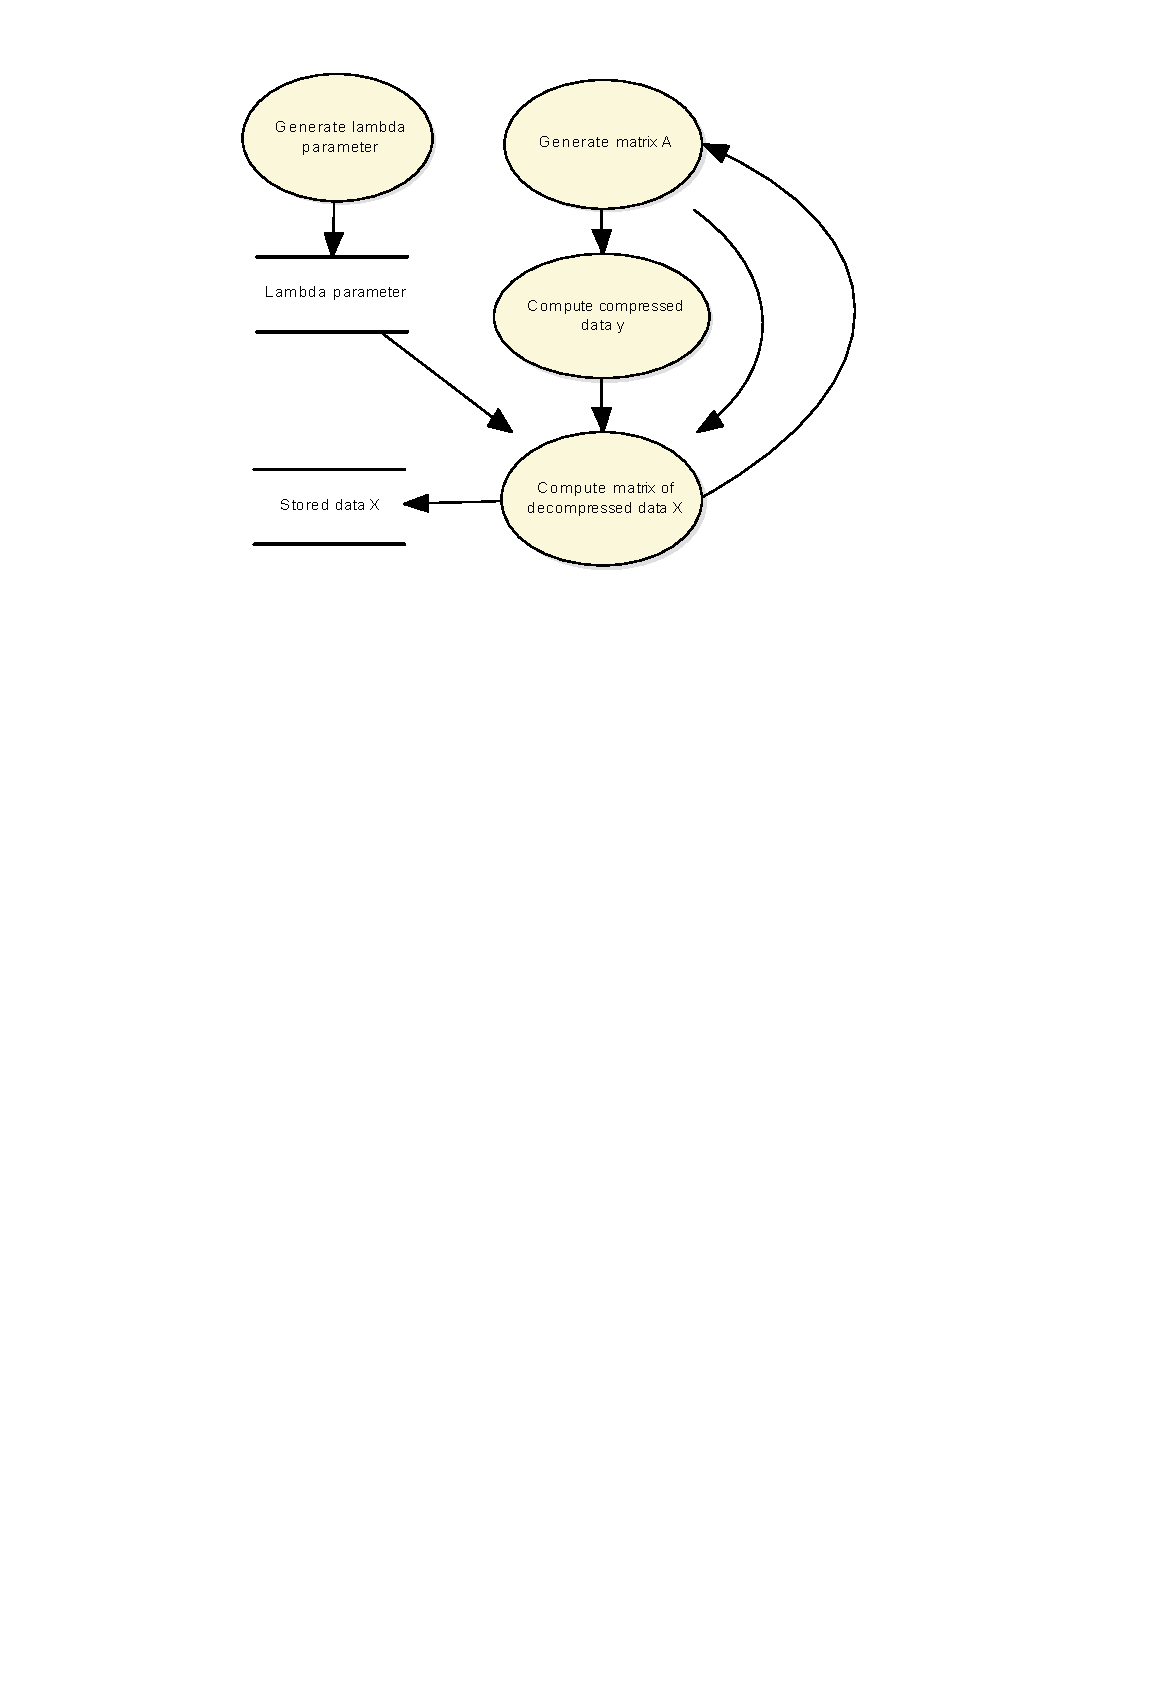
\includegraphics[scale=0.8]{obr/mcsim.pdf}
	\end{center}
	\caption{Simulace Monte Carlo}
	\label{fig:mcSim}
\end{figure}

Protože jde pouze o opakované provádění testovaného algoritmu, je tato simulace velice jednoduchá na realizaci. Základní algoritmus lze popsat jednoduchým diagramem \ref{fig:mcSim}. Nicméně jakákoliv takováto simulace má obrovskou nevýhodu a to je celkový čas simulace. Při větších datech může výpočet trvat i několik dní. V případě této konkrétní simulace se 100 prvky $\lambda$ a 1000 opakování trvala tato simulace pro $\left\| \cdot\right\|_{2}^{2} $ LASSO přes jedenáct hodin. Pro porovnání byl algoritmus upraven pro $\left\| \cdot \right\|_2 $ LASSO a takováto simulace již trvala přes tři dny. Jelikož je vše realizováno pomocí vývojového prostředí a jazyku MATLAB, jednou z možností bylo vytvořit knihovní funkce v jazyku C nebo C++, aby se docílilo zrychlení algoritmu a využít této knihovny funkcí místo skriptů v MATLABu. Nicméně toto by bylo velice zdlouhavé řešení a špatně testovatelné kvůli možným chybám. Z tohoto důvodu byla nalezena další možnost a to neřešit celkový čas. Následně tedy bylo toto řešení simulace rozšířeno o další blok, kterým se docílí toho, že výsledky nebudou ztraceny při nečekaných událostech.

\section{Interakce s uživatelem}
Onou nalezenou možností, jak je zmíněno v předchozí kapitole, je průběžné zálohování výsledků. První varianta této funkce byla realizována pomocí jednoduché tabulky, kam byly ukládány pouze výsledky. Nicméně s takto zálohovanými výsledky již nebylo možné pokračovat v simulaci. Z tohoto důvodu byla vytvořena struktura v MATLABu, viz \ref{fig:struktura}.

\begin{figure}[!ht]
	\begin{center}
		\includegraphics[scale=0.6]{obr/structure.pdf}
	\end{center}
	\caption{Struktura dat}
	\label{fig:struktura}
\end{figure}

Takto připravená struktura je již zálohována a následně také obnovována ze souboru. Pro tyto účely bylo využito funkcí \uv{save} a \uv{load}, jež jsou součástí standardní instalace prostředí MATLAB. Obě tyto funkce jsou navíc podmíněny a to tak, že v případě funkce \uv{save} je do konce simulace ukládána i dočasná iterační proměnná. Jak je již patrné právě tato proměnná by měla být také obnovena při načítání dat. S takto připraveným zálohováním zbývá vytvořit jediné a to komunikace s uživatelem. Tato komunikace byla vytvořena tak, že skript prochází umístění, kde se nachází a pokud nalezne soubor s příponou \uv{.mat}, je spolu s indexem vypsán na obrazovku a je tak vytvořeno textové menu. Následně uživatel volí soubor, se kterým chce pracovat pomocí tohoto indexu. Po zvolení souboru se obnoví uložená struktura dat a pokud soubor obsahuje i iterační proměnnou, tak i ta je obnovena a to tak, že je zároveň zvýšena o $1$ a to proto, že ukládání struktury probíhá po použití algoritmu pro všechny parametry $\lambda$, nikoliv před. Kdyby se tato proměnná neinkrementovala, tak by došlo ke zbytečnému průběhu a výpočetní čas by byl plýtván právě na tento průběh.

Dalším rozšířením, které bylo realizováno je možnosti upozornění uživatele na dokončení simulace. Jednou z možností bylo využít e-mailových služeb přímo v prostředí MATLABu, nicméně toto by mělo tu nevýhodu, že by nešlo spustit současně více různých skriptů, které by toho využívaly a posílaly tak informace o svém průběhu více uživatelům. Aby nebylo zapotřebí využívat prostředí MATLABu, byl vytvořen jednoduchý skript v jazyku Python a využitím služby Pushbullet. Jedná se o službu, která umožňuje odesílat zprávy, případně i malé soubory. Za pomoci dokumentace a rozhraní Pushbullet byl vytvořen skript, který přijímá na vstupu argumenty pro název a tělo zprávy. Takto převzaté informace se naformátují do hlavičky POST dotazu spolu s přístupovým tokenem konkrétního uživatele. Pokud je takto skript vykoná, uživatel dostane okamžitě upozornění na všechna svá zařízení a to buď pomocí mobilní aplikace nebo webového prostředí.
\section{Výsledek pro $l_{2}^{2}$ LASSO}
S takto připravenou simulací již lze přistoupit k samotnému použití. Na začátku simulace je důležité zvolit několik parametrů: počet parametrů $\lambda$ a jejich rozsah, počet prvků původních dat $x$, počet řádků měřících matic $A$ a také počet opakování průběhu algoritmu. Toto nastavení je také uloženo ve struktuře, jak bylo vysvětleno v předchozí kapitole. Po ukončení často velice dlouhé simulace je získána empirická závislost kvadratické chyby nalezeného řešení od skutečného pro každý prvek z vektoru parametrů $\lambda$. Nejčastěji lze získat křivku podobnou následujícímu grafu: 

\begin{figure}[!ht]
	\begin{center}
		\includegraphics[scale=0.7]{obr/l22simulation.pdf}
	\end{center}
	\caption{Simulace pro $l_{2}^{2}$ LASSO}
	\label{fig:l22sim}
\end{figure}
\chapter{Výsledky}
\label{ch:vysledky}
Tato kapitola se bude zabývat získáním výsledků pomocí naimplementovaných algoritmů, odvozením vzorců pro výpočet analytické chyby vybraného, ale i obdobného, problému a porovnáním takto získaných výsledků. 

Jelikož odvození vztahu pro výpočet kvadratické chyby nalezeného řešení od původních dat podle parametru $\lambda$ pro $\left\| \cdot \right\|_{2}^{2} $ LASSO je velice obtížné, je zvolen jiný přístup, který je využíván běžně pro tento problém. Tento přístup využívá toho, že lze použít jinou variantu tohoto optimalizačního problému a to $\left\| \cdot \right\|_{2}$ LASSO, pro kterou je analýza daleko jednodušeji proveditelná a následně na tuto analýzu aplikovat mapovací funkci. Nicméně toto nás vrací zpět na začátek zadání a proto budou jednotlivé kroky popsány v jednotlivých podkapitolách. 
\section{Rekonstrukce dat pomocí CVX knihoven a Monte Carlo simulace}
Velice důležitým prvním krokem je samotná rekonstrukce dat. Jelikož tato varianta problému LASSO nemusí mít shodné vlastnosti jako doposud použité $\left\| \cdot \right\|_{2}^{2} $ LASSO. I samotný gradient této funkce je velice náročný na výpočet a nelze ani nic před počítat před samotným prováděním algoritmu, viz \ref{eq:l2Grad}.

\begin{equation} \label{eq:l2Grad}  \tag{Vzorec \theVzorce}
-A^{T} \times \frac{\left(y-A \times x\right)}{\left\| y - A \times x\right\|_{2} }
\end{equation}
\myequations{\ref{eq:l2Grad} - Gradient $l_2 $ LASSO}
\stepcounter{Vzorce}

Z tohoto důvodu bylo využito open source knihoven CVX. Tyto knihovny jsou primárně zaměřené na modelování konvexních optimalizací a tak využívají daleko přesnějších a rychlejších algoritmů než bylo použito v této bakalářské práci. 

Po přidání tohoto balíku do vývojového prostředí MATLAB lze použít modelovacího jazyka pro vytvoření jednoduchého skriptu, který bude provádět totéž, co bylo dosud implementováno. Jelikož se jedná o snadno použitelný modelovací jazyk, není náročné implementovat skript, který bude minimalizovat vybraný problém a může vypadat následovně: 

\begin{lstlisting}
for i = 1:pocet_opakovani
    y = A*x;
    for j = 1:length(lambda)
        cvx_begin quiet
	    variable x_n(pocet_prvku)
	    minimize((norm(y-A*x_n,2)+lambda(j)*norm(x_n,1)))
	    cvx_end
    end
end
\end{lstlisting}

Jak je vidět, tak balík knihoven CVX opravdu velice výrazně zjednodušuje realizaci vybraného problému. Vše začíná příkazem \uv{cvx\_begin}, který deklaruje začátek deklarací a funkcí. Zde je využito varianty s parametrem \uv{quiet}, aby byl potlačen výpis částečných výsledků během opakování této části skriptu. Následně je deklarována proměnná $x_n$, přes kterou se minimalizuje zadaný problém a to o předem daném počtu prvků. Poté již následuje příkaz \uv{minimize}, kterému se deklaruje funkce, kterou chceme minimalizovat. V této funkci je využita standardní funkce \uv{norm} a to jak pro zápis $\left\| y - A \times x_n\right\|_2$, tak pro $ \left\| x \right\|_1  $, která je ještě zvětšena, resp. zmenšena, j prvkem z vektoru parametrů $\lambda$. Vše je uzavřeno druhou polovinou párového příkazu a to příkazem \uv{cvx\_end}.

Takto připravený skript vytváří empirické pozorování, jako je již vytvořeno v kapitole \ref{ch:simulace}. Získáváme tak graf \ref{fig:l2}, který se v několika bodech podobá již dříve získaným grafům \ref{fig:l22sim}. Pro jednoduchost zde není uvažována varianta s náhodným šumem, jako v předešlém případě.

\begin{figure}[!ht]
	\begin{center}
		\includegraphics[scale=0.7]{obr/l2.pdf}
	\end{center}
	\caption{Kvadratická chyba řešení problému $l_2$ LASSO}
	\label{fig:l2}
\end{figure}

V porovnáním s kvadratickou chybou problému $l_{2}^{2}$ LASSO, viz \ref{fig:l22sim}, tak lze vidět, že optimální hodnota je velice podobná optimální hodnotě v předchozím případě. Zbývá tedy zjistit analytickou předpověď pro tento problém.

\section{Aplikování mapovací funkce na analytickou předpověď  $l_{2}$ LASSO}

\section{Porovnání empirických výsledků a analytické předpovědi}
\chapter{Závěr}
\label{ch:end}

\renewcommand{\bibname}{Seznam použité literatury}
\begin{thebibliography}{99}
\bibitem{convexOptimization} BOYD, Stephen P a Lieven VANDENBERGHE. Convex optimization. New York: Cambridge University Press, 2004. ISBN 0521833787.
\bibitem{homotopy}Z. Koldovský a P. Tichavský, "A Homotopy Recursive-in-Model-Order Algorithm for Weighted Lasso," Proc. of the 41st IEEE International Conference on Audio, Speech, and Signal Processing (ICASSP 2014), Florence, Italy, pp. 4151-4155, May 2014.
\end{thebibliography}
\clearpage
\appendix
\chapter*{Přílohy}
\captionsetup[figure]{list=no}
\begin{appendices}
	\section*{Příloha A: Obsah přiloženého CD}
	\label{appA}
	\newpage
	\section*{Příloha B: Finální podoba algoritmu}
		\begin{figure}[!ht]
			\begin{center}
				\includegraphics[scale=0.9]{obr/finalAlg.pdf}
			\end{center}
			\caption{Diagram finálního algoritmu}
			\label{fig:finalAlg}
		\end{figure}
\end{appendices}
\end{document}
